\documentclass[grad,numbers]{coppe}
\usepackage{amsmath, amssymb, diagbox}
\usepackage{hyperref}
\usepackage[utf8]{inputenc}
\usepackage[brazil]{babel}
\usepackage[T1]{fontenc}
\usepackage{graphicx}
\usepackage[cache=false]{minted}

\makelosymbols
\makeloabbreviations

\begin{document}
  \title{Análise de Notícias do Mercado Financeiro Utilizando Processamento de Linguagem Natural e Aprendizado de Máquina Para Decisões de Swing Trade}
  \foreigntitle{Financial Market News Analysis Using Natural Language Processing and Machine Learning for Swing Trade Decisions}
  \author{Lucas}{Gama Canto}
  \advisor{Prof.}{Heraldo Luís}{Silveira de Almeida}{D.Sc.}

  \examiner{Prof.}{[TODO]Nome do Primeiro Examinador Sobrenome}{D.Sc.}
  \examiner{Prof.}{[TODO]Nome do Segundo Examinador Sobrenome}{Ph.D.}
  \examiner{Prof.}{[TODO]Nome do Terceiro Examinador Sobrenome}{D.Sc.}
  
  \department{ECA}
  
  \date{03}{2020}

  \keyword{Aprendizado de Máquina}
  \keyword{Processamento de Linguagem Natural}
  \keyword{Mercado Financeiro}

  \maketitle

  \frontmatter
  
  \makecatalog
  
  \dedication{Ao povo brasileiro, pela total contribuição em minha graduação.}

  \chapter*{Agradecimentos}

	  \paragraph{}Gostaria de agradecer a todas as pessoas e situações que tornaram este momento possível. Em especial, meus pais Benedita e Manoel, pelo suporte e esforço incondicional em apoiar minha decisão de vir estudar engenharia no Rio de Janeiro, aos professores da graduação, que me fizeram evoluir no âmbito acadêmico, profissional e pessoal, em especial ao meu orientador e professor Heraldo, que não mediu esforços para me ajudar neste trabalho, e aos amigos que me apoiaram e participaram do meu processo de graduação.

  \begin{abstract}

	  \paragraph{}Com o objetivo de automatizar análises fundamentalistas de mercado, o uso de tecnologia para processamento de texto vem sendo utilizado constantemente no meio acadêmico\cite{nlp-academics} e profissional\cite{nlp-industry}. De forma a contribuir para este campo em crescimento, este trabalho discorre um estudo acerca da criação de modelos preditivos sobre a valorização ou desvalorização de ações na bolsa de valores do Brasil (B3, antiga Bovespa) a partir de notícias sobre o mercado brasileiro de forma a auxiliar decisões de Swing Trade, ou seja, compra e venda de ações dentro de uma janela de tempo maior que um dia.
	  \paragraph{}Para isto, o presente projeto utiliza o framework PyText, que se baseia em conceitos de Aprendizado de Máquina, Redes Neurais e Processamento de Linguagem Natural de forma a desenvolver modelos preditivos com a tarefa de classificação textual.

  \end{abstract}

  \begin{foreignabstract}

	  \paragraph{}In order to automate fundamental market analysis, the use of text processing technology has been constantly used in academic\cite{nlp-academics} and professional\cite{nlp-industry} means. To contribute to this growing field, this paper discusses a study about the creation of predictive models regarding the valuation or devaluation of shares on the Brazilian stock exchange (B3, former Bovespa) based on news about the Brazilian market in order to assist Swing Trade decisions, that is, buying and selling stocks within a time window longer than one day.
	  \paragraph{}To this end, the present project uses the PyText framework, which is based on Machine Learning, Neural Networks and Natural Language Processing concepts in order to develop predictive models with the task of textual classification.

  \end{foreignabstract}

  \tableofcontents
  \listoffigures
  \listoftables
  \printlosymbols
  \printloabbreviations

  \mainmatter
%  \doublespacing
	\chapter{Introdução}
		
		\section{Tema}
			\paragraph{}O tema deste trabalho se resume no estudo da criação de modelos preditivos de modo que estes possam prever a valorização ou desvalorização de ações da bolsa de valores por meio do processamento de notícias do mercado brasileiro.
			\paragraph{}Deste modo, o problema a ser abordado é a identificação de quando uma notícia pode impactar positivamente ou negativamente a variação de preço de ações de forma automatizada.
			
		\section{Delimitação}
			\paragraph{}Este trabalho se restringe ao processamento de texto em português brasileiro, tendo como foco a predição da variação de preço das ações que fazem parte da bolsa de valores do Brasil, a B3. Pela indisponibilidade de dados sobre notícias brasileiras contendo a informação do horário de lançamento da notícia, o projeto mira em predições dentro de uma janela de tempo maior que um dia, de forma a auxiliar decisões de Swing Trade, isto é, operações de compra e venda de ações numa janela de tempo maior que um dia.
			\paragraph{}Além disso, o estudo se baseia na ferramenta PyText, um framework recentemente desenvolvido pelo Facebook que providencia modelos de processamento de linguagem natural de última geração através de uma interface simples e extensível\cite{pytext-paper}.
		
		\section{Justificativa}
			\paragraph{}Diante do crescente número de investidores na bolsa de valores no Brasil, nota-se uma maior preocupação da população brasileira acerca da busca por independência financeira e fontes alternativas de renda com o intuito de contribuir à economia familiar, previdência, ou mesmo utilizar este método como fonte principal de renda\cite{bovespa-investors-growth}.
			\paragraph{}Ao mesmo tempo, estudos associados à inteligência artificial, aprendizado de máquina e processamento de linguagem natural continuam emergindo no meio acadêmico e auxiliando o meio profissional como nunca antes, incluindo o mercado financeiro\cite{ai-in-financial-growth}.
			\paragraph{}Através destes dois fatores, o presente trabalho busca contribuir para a difusão do estudo e uso de algumas destas tecnologias sobre um assunto que gradualmente se encontra dentro do interesse da população brasileira e que colabora para uma possível instauração de uma cultura de economia e independência financeira no Brasil.
		
		\section{Objetivos}
			\paragraph{}O objetivo geral do presente trabalho é de analisar modelos preditivos associados ao mercado financeiro que possam ser construídos a partir do framework PyText, tendo como objetivos específicos, apresentar: (1) A busca por dados de notícias e do histórico da bolsa de valores; (2) A lógica utilizada para a união destes dados de forma a construir os conjuntos de dados utilizados no treinamento dos modelos; (3) O pré-processamento dos conjuntos de dados; (4) As possíveis configurações do framework utilizado de forma a obter a melhor performance; (5) O detalhamento e a análise dos modelos finais encontrados.
		
		\section{Metodologia}
			\paragraph{}O trabalho teve início a partir da procura por bases de dados de notícias associadas ao mercado brasileiro e escritas em português do Brasil, seguida pela obtenção do histórico das variações de preço dos ativos que compõem o iBovespa. Após isto, o histórico foi filtrado de forma a manter as informações dos 5 ativos mais significativos e das varições destes ativos que ocorreram dentro da mesma janela de tempo das notícias obtidas. Em seguida, estes dados foram unidos de forma a obter 5 conjuntos de dados para cada ativo, cada um levando em consideração uma diferente janela de tempo para indicar a valorização: de 1 a 5 dias.
			\paragraph{}Logo após, houve a etapa de pré-processamento do corpo das notícias de forma a remover possíveis ruídos e facilitar a etapa de treinamento, sem perda de contexto do conteúdo. Com os conjuntos de dados prontos, foram feitos testes no PyText com o objetivo de definir a melhor configuração possível para a natureza dos dados, e assim obter a melhor performance.
			\paragraph{}Por fim, os testes finais de cada modelo gerado foi detalhado e analisado para permitir uma conclusão e avaliação do processo como um todo.

		\section{Descrição}
			\paragraph{}O capítulo 2 apresenta toda a fundamentação teórica utilizada como base para o projeto a partir de uma breve descrição de como a bolsa de valores funciona seguida de explicações sobre Aprendizado de Máquina, Processamento de Linguagem Natural, Redes Neurais e o framework Pytext.
			\paragraph{}No capítulo 3 é detalhado todo o processo executado para obtenção do conjunto de notícias e do histórico da B3, seguido do pré-processamento realizado nestes dois conjuntos e a criação dos conjuntos de dados finais utilizados para o treino, cada um associado a um ativo e uma janela de tempo específica.
			\paragraph{}Os detalhes das configurações utilizadas no PyText e o treinamento em si é especificado no capítulo 4, onde há uma discussão acerca dos parâmetros encontrados para a geração de modelos mais performáticos, além das métricas finais encontradas para cada modelo gerado.
			\paragraph{}Por fim, o capítulo 5 apresenta uma conclusão acerca dos modelos encontrados seguido por sugestões que futuramente podem ser aplicadas para a evolução do tema e uma possível melhora de desempenho dos modelos preditivos.
			\paragraph{}O código desenvolvido para o pré-processamento e geração dos conjuntos de dados e arquivos de configurações do PyText utilizados para a geração dos modelos podem ser encontrados no repositório do github referenciado em \cite{github}.
   
  \chapter{Fundamentação Teórica}
  
  \section{Bolsa de Valores e Ações}
  	\paragraph{}A Bolsa de Valores é um lugar centralizado onde, além de abranger outros tipos de investimento, se negociam ações (também chamados de ativos ou papéis), isto é, parcelas do capital social de empresas de capital aberto. Atualmente a B3 (Brasil, Bolsa, Balcão) é a Bolsa de Valores oficial do Brasil que em 2017 atingiu a 5ª posição das maiores bolsas de mercados de capitais do mundo em valor de mercado, com um patrimônio de US\$ 13 bilhões\cite{b3-patrimonio}.
  	\paragraph{}As ações são negociadas diariamente a partir das ordens de compra e venda emitidas pelas corretoras durante o pregão eletrônico, que na B3, funciona em dias úteis das 10:00 às 17:00.
  	\subsection{Preços de Ações}
  		\paragraph{}O preço de um ativo na Bolsa de Valores pode ser determinado por diversas razões que podem se relacionar entre si, entre essas, pode-se destacar a lei da oferta e demanda, perspectivas de crescimento da empresa associada ao papel e especulação. A previsibilidade acerca de movimentações no mercado de ações normalmente pode ser baseada em Análise Técnica (AT - estudo dos movimentos do mercado baseado em métricas como preço, volume e taxa de juros\cite{analise-tecnica}), Análise Fundamentalista (AF - estudo feito a partir de resultados financeiros e operacionais, indicando a saúde da empresa\cite{analise-fundamentalista}) ou numa junção destes dois conceitos.
  		\paragraph{}A validade da previsibilidade destas movimentações são questionadas por críticas com base na Hipótese do Mercado Eficiente (HME) e seus três níveis definidos em \cite{emh}:
			\begin{itemize}
				\item HME fraca: Afirma que os preços refletem totalmente a informação contida na sequência histórica dos preços. Ou seja, a AT não consegue prever os movimentos futuros pois os preços passadas só podem descrever o presente.
				\item HME semi-forte: Afirma que os preços presentes não só refletem toda a sequência histórica de preços mas também toda informação pública sobre as organizações associadas ao ativo em questão. Neste nível de eficiência, a AF também não seria capaz de prever movimentos futuros, pois toda informação como demonstrativos de resultados ou análises orçamentárias refletiria apenas o preço presente.
				\item HME forte: Neste nível, é afirmado que \textit{toda} informação conhecida sobre as organizações é totalmente refletida pelo preço presente, logo, nem mesmo aqueles com informações privilegiadas podem utilizar isto como ferramenta para prever preços futuros.
			\end{itemize}
 			\begin{figure}[h]
 				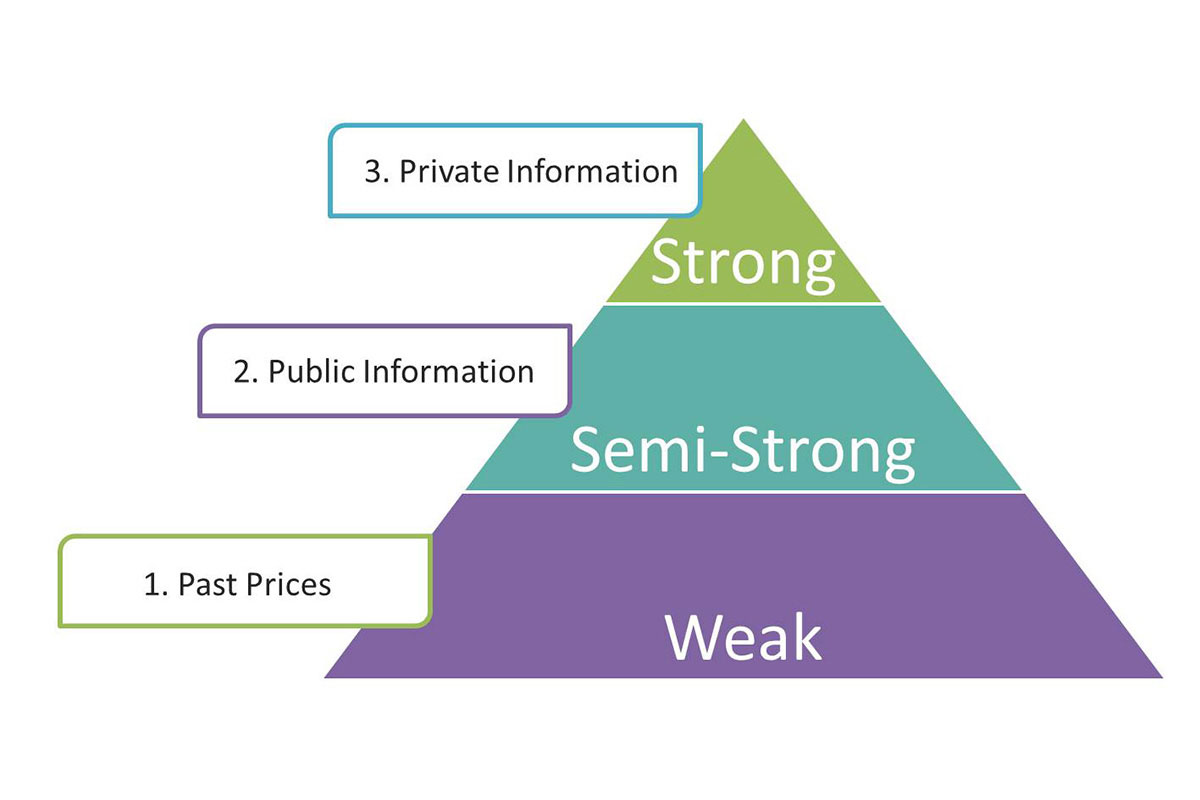
\includegraphics[width=13cm]{emh.jpg}
 				\caption{Os três níveis da HME, cada nível adiciona um tipo de informação cujo com o qual não seria possível prever um movimento de preço no mercado\cite{emh-article}.}
 				\label{fig:emh}
 			\end{figure}
 			\paragraph{}Não há uma reposta correta perante a validade da HME. Porém, muitos acadêmicos acreditam, pelo menos, na HME fraca\cite{emh-br}, fazendo com que, em algumas ocasiões, seja preferível a utilização da AF, ou seja, a análise de resultados financeiros, relatórios anuais e notícias divulgadas acerca do mercado financeiro.
 			
		\subsection{Índice de Bolsa de Valores}
			\paragraph{}Com objetivo de parametrizar algumas informações intrínsecas às bolsas, estas disponibilizam diversos índices. O principal índice da B3 é o Ibovespa, que é formado pelos ativos com maior volume negociado na bolsa nos últimos meses e indica, de forma resumida, o desempenho das ações negociadas na B3. Por ser um indicador principal, muitos fundos de investimento baseados no mercado de ações estão atrelados ao Ibovespa, contribuindo para a atratividade destes ativos de maneira geral.
			\begin{table}[h]
				\caption{Os 5 ativos com o maior volume e participação na B3, associados ao Ibovespa\cite{carteira-bovespa}.}
				\label{tab:ibovespa-5bigger}
				\centering
				{\footnotesize
					\begin{tabular}{|c|c|c|c|}
						\hline
						Código & Ação & Qtde. Teórica & Part.(\%)\\
						\hline
						ITUB4 &  Itaú Unibanco & 4.738.562.684 & 9,095 \\
						PETR4 &  Petrobras & 4.520.185.835 & 7,038 \\
						BBDC4 &  Bradesco & 3.873.597.664 & 7,028 \\
						VALE3 &  Vale S.A. & 3.147.743.563 & 8,414 \\
						ABEV3 &  AMBEV & 4.344.066.764 & 4,173 \\
						\hline
				\end{tabular}}
			\end{table}
			 
  \section{Aprendizado de Máquina}
  	\paragraph{}Pode-se definir Aprendizado de Máquina como o campo de estudo de algoritmos com o objetivo de fazer com que computadores possam agir sem serem explicitamente programados para fazer determinada tarefa. São algoritmos que analisam dados e aprendem com eles, gerando um modelo preditivo que pode fornecer uma predição de algo on mundo.
  	\paragraph{}Outra definição dada por Tom M. Mitchell\cite{ml-mitchell} fala que o campo de Aprendizado de Máquina busca responder a pergunta: ``Como podemos construir sistemas de computadores que possam automaticamente melhorar através de experiência e quais são as leis fundamentais que governam todo este processo de aprendizado?''. Outra definição do mesmo autor\cite{ml-mitchell-book} diz que ``Um programa de computador é dito aprender com a experiência E em respeito a uma tarefa T e medida pelo desempenho P se o seu desempenho em T, medido por P, melhora com a experiência E''. Neste conceito, se fosse desejado um programa de computador que aprendesse a classificar e-mails como spam ou não, por exemplo, poderíamos fazer a seguinte associação:
  	\begin{itemize}
  		\item E = A experiência de ver o usuário classificar emails como spam ou não.
			\item T = A tarefa de classificar os emails.
			\item P = O número ou fração de emails corretamente classificados como spam/não spam
  	\end{itemize}
  	\paragraph{}Geralmente, os algoritmos de Aprendizado de Máquina podem ser divididos em dois tipos: Aprendizado Supervisionado e Aprendizado Não Supervisionado.
  	\subsection{Aprendizado Supervisionado}
  		\paragraph{}Neste tipo, o algoritmo é inicialmente servido por uma série de dados rotulados cujo resultado já é conhecido. A ideia e que o algoritmo aprenda a criar uma estratégia para chegar ao resultado baseando-se nesses dados de modelo inicial. O aprendizado supervisionado pode ser dividido em problemas de regressão ou classificação.
  		\subsubsection{Problema de Regressão}
	  		\paragraph{}Neste tipo de problema, os dados de entrada (parâmetros) são mapeados em uma função contínua. Por exemplo, um algoritmo cujo objetivo fosse prever o preço dos imóveis na cidade do Rio de Janeiro baseando-se em dados como área útil, bairro, número de vagas na garagem, etc é considerado como um problema de regressão, pois o resultado final será um número contínuo, neste caso, o preço dos imóveis.
  		\subsubsection{Problema de Classificação}
  			\paragraph{}Neste caso, os parâmetros são mapeados de forma a classificar os dados em categorias distintas. Por exemplo, um algoritmo utilizado para prever se um tumor é benigno ou maligno a partir de dados como o tamanho, rugosidade do tumor e idade do paciente é considerado um problema de classificação, pois o resultado final será a categoria na qual o tumor pertence.
  			\paragraph{}Os problemas de classificação muitas vezes apresentam desbalanceamento de classes no conjunto de dados utilizado para o treinamento do modelo, ou seja, o conjunto de dados pode apresentar poucas amostras de uma determinada classe em relação às outras envolvidas, o que pode ocasionar falhas na predição da classe minoritária.
  			\paragraph{}De forma a corrigir tal problema, existem algumas técnicas que podem ser baseadas em dois conceitos: \textit{Undersampling} e \textit{Oversampling}. A primeira se resume na remoção de amostras das classes majoritárias, e a segunda, no acréscimo de amostras da classe minoritária a partir das amostras já existentes no conjunto, de forma a se obter um conjunto de dados balanceados.
  			\newpage
  			\begin{figure}[h]
  				\centering
  				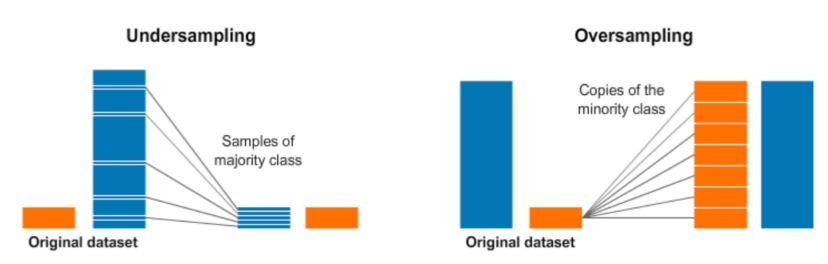
\includegraphics[width=13cm]{os_and_us.jpg}
  				\caption{Exemplos das estratégias de \textit{Undersampling} e \textit{Oversampling} em um problema de classificação de 2 classes desbalanceadas\cite{os_and_us}.}
  				\label{fig:os_and_us}
  			\end{figure}
  			\paragraph{}Entretanto, estas técnicas podem gerar alguns efeitos negativos, como por exemplo, a demasiada diminuição do conjunto de dados como um todo no \textit{Undersampling}, o que prejudica o aprendizado. No caso do \textit{Oversampling}, pode-se gerar um maior efeito de sobre-ajuste no modelo preditivo, isto é, pela falta de generalização, o modelo consegue prever muito bem amostras do conjunto de dados de treino, mas se mostra ineficaz ao prever dados de teste.
		\subsection{Aprendizado Não Supervisionado}
			\paragraph{}Neste tipo de aprendizado, não existe um conjunto inicial de dados e resultados, ou seja, nos permite abordar problemas onde temos pouca ou nenhuma ideia do que nossos resultados devem aparentar. Um exemplo, seria um algoritmo onde, utilizando uma coleção de 1000 artigos publicados por uma universidade, fizesse um agrupamento desses artigos, baseando-se em diferente variáveis como frequência de palavras semelhantes, número de paginas, etc.
		\subsection{Avaliação de Desempenho}
			\paragraph{}A avaliação de desempenho de um modelo preditivo pode ser realizada através de diversas métricas que são medidas diante de uma previsão do modelo sobre um conjunto de dados de teste, logo, existe uma necessidade em dividir o conjunto de dados inicial em dados de treino e dados de teste.
			\paragraph{}Não existe um modo ideal de dividir o conjunto de dados, o tamanho do conjunto de treino normalmente é maior que o de teste, de modo que este consiga abranger mais generalizações acerca dos parâmetros do modelo. Assim, algumas proporções são mais comumente usadas, como 60/40, 75/25 e 80/20, proporção baseada no Principio de Pareto que afirma que, 80\% das saídas/consequências vem de 20\% das entradas/causas\cite{pareto_principle}. Levando em consideração o escopo de Aprendizado de Máquina, podemos dizer que 20\% pode mapear 80\% do conjunto de dados.
			\paragraph{}Além disso, em modelos mais simples, também existe a possibilidade de utilizar a Validação Cruzada, uma técnica que separa o conjunto de dados em subconjuntos exclusivos e diferentes e alguns destes subconjuntos são utilizados para treino e outros para teste, de forma iterativa. Um dos métodos de validação cruzada mais famosos é o \textit{k-fold}, onde o conjunto de dados é separado em $k$ subconjuntos e o treino é realizado $k$ vezes, cada vez utilizando um subconjunto diferente para teste e o resto para treino\cite{k-fold}. No final, as métricas de avaliação são definidas como a média diante dos $k$ subconjuntos.
			\subsubsection{Métricas}\label{sec:metricas}
				\paragraph{}As métricas utilizadas para avaliação dependem do tipo de problema. Por exemplo, em problemas de regressão é comum utilizar o erro quadrático médio\cite{regression-loss}. Nos problemas de classificação, é comum utilizar as seguintes medidas: Acurácia, Precisão, Cobertura e a Medida F1:
				\begin{itemize}
					\item Acurácia: É a medida que define a assertividade do modelo em geral, se resume na porcentagem de acertos dentre todas as previsões feitas no conjunto de teste.
					\begin{equation*}
						A = \frac{\text{Número total de acertos}}{\text{Número total de palpites}}
					\end{equation*}
					\item Precisão: Medida de assertividade referente a uma classe específica. É a porcentagem de acertos dentre todos os palpites de uma classe.
					\begin{equation*}
						P_X = \frac{\text{Número total de acertos da classe X }}{\text{Número total de palpites da classe X}}
					\end{equation*}
					\item Cobertura: Porcentagem de palpites certos dentro do número de amostras de uma classe específica.
					\begin{equation*}
						C_X = \frac{\text{Número total de acertos da classe X }}{\text{Número total de amostras da classe X}}
					\end{equation*}
					\item  Medida F1: Média harmônica entre Precisão e Cobertura.
						\begin{equation*}
						F1_X = 2\frac{P_X C_X}{P_X + C_X}
						\end{equation*}
				\end{itemize}
  
  \section{Redes Neurais}
	  \paragraph{}Redes neurais são estruturas matemáticas baseadas no funcionamento do cérebro humano. O campo que estuda a aplicação de redes neurais com várias camadas de processamento em métodos de Aprendizado de Máquina é chamado de Aprendizagem Profunda (do inglês, \textit{Deep Learning}). Em sua forma mais simples, uma rede neural contém três camadas: entrada (\textit{input layer}), camada oculta (\textit{hidden layer}) e saída (\textit{output layer}), onde a camada oculta pode ser única ou múltipla. Cada camada é composta por neurônios, também chamados de nós.
	  \begin{figure}[h]
	  	\centering
	  	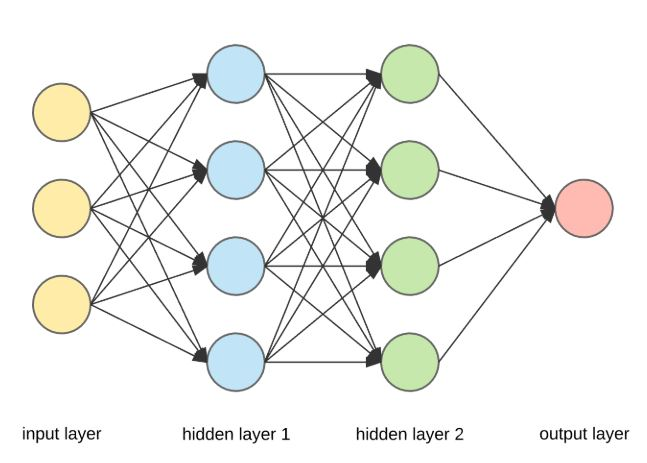
\includegraphics[width=10cm]{nn1.jpg}
	  	\caption{Exemplo de rede neural com duas camadas ocultas\cite{nn1-example}.}
	  	\label{fig:nn1-fig}
	  \end{figure}
  	\paragraph{}Cada nó de uma rede neural representa uma abstração matemática, esta é definida pela função de ativação (\textit{Activation Function}) que recebe o somatório das entradas (\textit{Inputs}) multiplicadas por seus respectivos pesos e mais um viés (\textit{Bias}).
  	\begin{figure}[h]
  		\centering
  		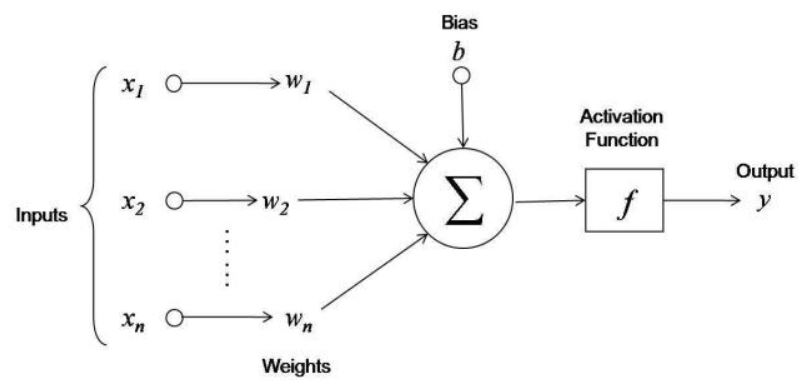
\includegraphics[width=11cm]{nn2.jpg}
  		\caption{Neurônio de uma rede neural\cite{nn2-example}.}
  		\label{fig:nn2-fig}
  	\end{figure}
  	\paragraph{}Durante a etapa de treinamento, estes pesos são ajustados de forma que se obtenha saídas iguais ou suficientemente próximas às saídas do conjunto de dados utilizado para treino, isso pode acontecer através de diversas técnicas, sendo a \textit{backpropagation} umas das mais conhecidas, que utiliza descida de gradiente\cite{nn-raul-rojas} para minimizar a função custo determinada pelas entradas, viés, função de ativação e saída dos neurônios.
  	\paragraph{}Este modelo simples de rede neural com apenas uma camada oculta se chama \textit{Perceptron} e os modelos com múltiplas camadas são chamados de \textit{Multilayer Perceptron} (MLP). Apesar de terem significante poder preditivo, estas redes podem apresentar falhas, principalmente quando o número de camadas ocultas alcança um valor muito grande ou quando os dados de entrada apresentam uma alta dimensão. Mesmo após algumas tentativas de solucionar estas falhas das redes MLP, outras arquiteturas de redes neurais foram propostas.
	  \subsection{Redes Neurais Convolucionais}
		  \paragraph{}As Redes Neurais Convolucionais (\textit{Convolutional Neural Network - CNN}) foram desenvolvidas com o intuito de facilitar a classificação de dados de alta dimensão, como imagens e textos. Em um problema de classificação de imagem com uma rede MLP, cada pixel está diretamente ligado a uma entrada, ocasionando um vetor de entrada de alta dimensão. Em uma rede CNN, normalmente, este vetor de entrada sofre diversas reduções de dimensionabilidade dentro de três camadas: camada de convolução, camada de função de ativação e camada de \textit{pooling}.
		  \paragraph{}Na primeira camada, ocorre a convolução do dado de entrada com um filtro (\textit{kernel}), que também é treinado ao longo do treinamento de toda a rede.
		  \begin{figure}[h]
		  	\centering
		  	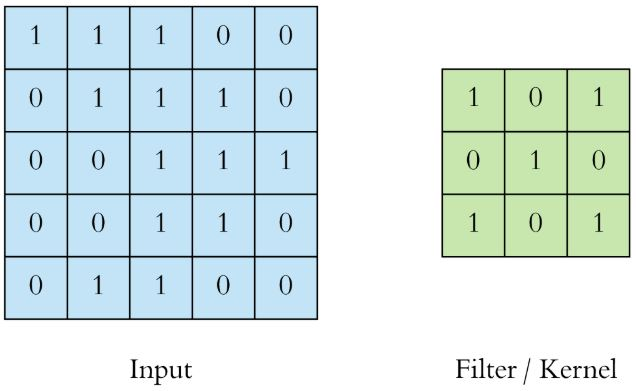
\includegraphics[width=10cm]{kernel.jpg}
		  	\caption{Exemplo de um dado de entrada e um \textit{kernel}\cite{kernel-example}.}
		  	\label{fig:kernel-fig}
		  \end{figure}
		  \newpage
	  	\begin{figure}[h]
	  		\centering
	  		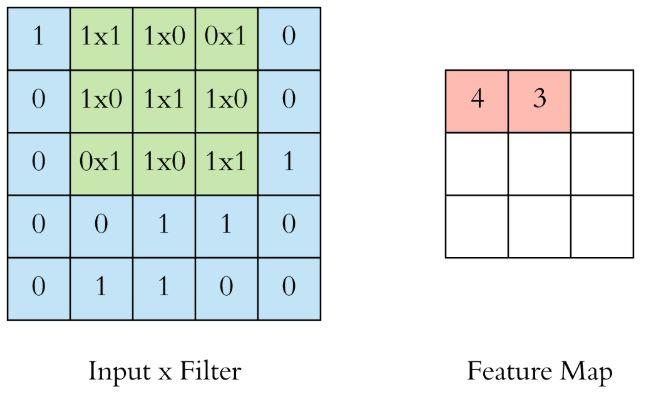
\includegraphics[width=10cm]{kernel2.jpg}
	  		\caption{Exemplo de convolução da imagem anterior\cite{kernel-example}.}
	  		\label{fig:kernel2-fig}
	  	\end{figure}
  		\paragraph{}Após esta etapa, o resultado da camada convolução passa por funções de ativação. Nestas, normalmente são atribuídas funções ReLU (\textit{Rectified Linear Unit}), análoga à função rampa, ou seja, valores menores que zero são zerados e o resto [e mantido. Por final, o resultado da camada de função de ativação passa pelo \textit{pooling} onde a redução de dimensibilidade pode ser feita através de diversas técnicas, sendo a \textit{max-pooling} a mais utilizada. Esta consiste em selecionar os maiores valores dentro de submatrizes de tamanho e espaçamento (passos) específicos, como indicado na figura abaixo.
  		\begin{figure}[h]
  			\centering
  			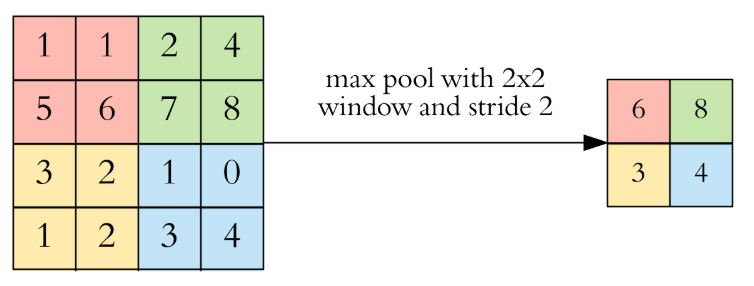
\includegraphics[width=11cm]{pooling.jpg}
  			\caption{Exemplo de \textit{max-pooling} utilizando uma submatriz de tamanho 2x2 e passo 2\cite{kernel-example}.}
  			\label{fig:pooling-fig}
  		\end{figure}
  		\paragraph{}Após estas camadas, o resultado pode ser utilizado na camada de entrada de uma rede comum, normalmente, uma rede MLP.
	  \subsection{Redes Neurais Recorrentes}
	  	\paragraph{}As Redes Neurais Recorrentes (\textit{Recurrent Neural Networks - RNN}) são redes que foram desenvolvidas principalmente para problemas associados à predição de sequência de dados, como a predição de palavras em um texto de entrada. TODO
  	\subsection{\textit{Dropout}}
  		\paragraph{}TODO
	  	
  \section{Processamento de Linguagem Natural}
  	\paragraph{}Processamento de Linguagem Natural (PNL) se resume ao campo de estudo das tecnologias utilizadas para ajudar computadores a entenderem a linguagem natural dos humanos, é também considerado uma subárea da Inteligência Artificial. Pode ser usado em diversas aplicações\cite{simple-nlp}, como por exemplo:
  	\begin{itemize}
  		\item Aplicativos de tradução de idioma, como o Google Translator
  		\item Processamento de palavras, que empregam PNL para a correção gramática
  		\item Resposta de Voz iterativa em call centers, de forma a responder adequadamente conforme a requisição de usuários
  		\item Assistentes pessoais, como OK Google, Siri, Cortana e Alexa
  	\end{itemize}
	  \paragraph{}Geralmente, o PNL abrange um pré-processamento de texto antes deste ser transformado em uma forma inteligível por computadores, de forma a remover ruídos ou facilitar o processamento, e isto pode ocorrer de diversas formas.
	  \subsection{Pré-processamento de Sintaxe}
	  	\paragraph{}A sintaxe se refere à forma de como as palavras se organizam em uma sentença para que se obtenha sentido gramatical. Estas são algumas técnicas de sintaxe que podem ser utilizadas no pré-processamento de texto:
	  	\begin{itemize}
	  		\item Stemização: É a transformação de palavras flexionadas para sua forma radical. Por exemplo, as palavras ``estudos'', ``estudar'' e ``estudando'' se transformariam apenas em ``estud'', mas a palavra ``tiver" se transformaria em ``tiv'' e ``tenho" se transformaria em ``tenh''.
	  		\item Lematização: Semelhante à Stemização, porém, a palavra é resumida para seu lema, fazendo com que se alcance um nível maior de abstração. Neste caso, tanto a palavra ``tiver'' como ``tenho'' se transformaria no lema  ``ter''.
	  		\item Remoção de \textit{stopwords}: A remoção de ``palavras de parada'', ou seja, palavras como ``a'', ``de'', ``o'', ``da'', ``que'', ``e'', ``do'' é útil pois, na maioria das vezes, não são informações importantes para construção do modelo.
	  	\end{itemize}
  	\paragraph{}Além destas, outra técnicas mais simples são utilizadas, como a transformação de caracteres maiúsculos para minúsculos.
  	\subsection{Representação Vetorial}
  		\paragraph{}Após o pré-processamento textual, diversas técnicas podem ser utilizadas para a transformação do texto em números. Uma das formas mais simples de se fazer isso é o \textit{Bag-of-Words} (BOW), que consiste em simbolizar textos de um conjunto de dados através de uma matriz na qual cada coluna é associada a uma palavra existente no conjunto de dados. Cada linha da matriz representa um texto e as variáveis indicam o número de ocorrências de uma palavra específica.
  		\begin{figure}[h]
  			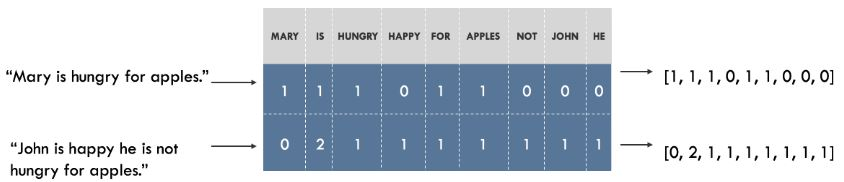
\includegraphics[width=15cm]{bow-example.jpg}
  			\caption{Exemplo de aplicação do \textit{Bag-of-Words}\cite{bow-example}.}
  			\label{fig:bow-example-fig}
  		\end{figure}
  		\paragraph{}Apesar da praticidade e simplicidade, o BOW apresenta alguns problemas, entre eles, a perda da informação de ordem das palavras e a alta dimensão da representação vetorial, fazendo com que muitos busquem outra alternativa... TODO
  		\subsubsection{Word2Vec}
  			\paragraph{}TODO
	  	
  
  
  \section{PyText}
  	\paragraph{}TODO
  	\subsection{Configuração}
  		\paragraph{}TODO
  	\subsection{Uso}
  		\paragraph{}TODO
  
  \chapter{Obtenção e Tratamento de Dados}
  	\paragraph{}Baseando-se na HME fraca e acreditando na possibilidade de realizar a análise fundamental de notícias sobre o mercado de forma autônoma, foi decidido o estudo acerca da criação de modelos preditivos de modo a prever a valorização, desvalorização ou preservação do preço de ativos da B3. Para isso, seria necessário a aquisição de um conjunto de dados de notícias e variações de preço de ativos grande o suficiente que relacionasse as datas/horários das notícias com as datas/horários das variações. Como um conjunto de dados que relacionasse diretamente notícias e variações de ativos não foi encontrado, ficou claro que seria necessário o cruzamento de dados a partir de dois conjuntos de dados diferentes.
  	\section{Conjunto de Dados de Notícias}
	  	\paragraph{}Inicialmente, foi preferido a escolha de realizar análises de forma a auxiliar decisões de \textit{Day Trade}, isto é, compra e venda de ações no mesmo dia, o que tornaria a informação de horário imprescindível. Isto logo se tornou inviável devido a falta de conjuntos de dados de notícias em português brasileiro com a informação de horário. Dentre os encontrados, todos continham apenas a data de lançamento da notícia.
	  	\paragraph{}Conjuntos de notícias em outros idiomas com a informação de horário foram encontrados, mas não foram utilizados devido ao foco do projeto que buscava analisar notícias do mercado brasileiro para auxiliar operações na B3. Também foram avaliadas as possibilidades de construir um \textit{web crawler} para obter notícias de sites como Folha de S. Paulo\cite{folha} ou InfoMoney\cite{infomoney} ou mesmo utilizar a API do Twitter\cite{twitter-api} para obter \textit{tweets} de contas associadas a veículos de notícias. A primeira possibilidade se mostrou complexa e demorada para o prazo estipulado para o projeto e a segunda foi impedida pelos limites que a versão gratuita da API propõe sobre os usuários. Sendo assim, foi decidido que a análise seria feita de forma a auxiliar decisões de \textit{Swing Trade}.
	  	\paragraph{}Dentre os conjuntos encontrados, foi escolhido o \textit{News of the brazilian newspaper}\cite{folha-news-dataset}, disponibilizado por um usuário do Kaggle, uma comunidade on-line de cientistas de dados. O conjunto contém 167,053 notícias categorizadas da página do jornal Folha no período entre janeiro de 2015 e setembro de 2017. O conjunto oferece as informações de, título, corpo, data, categoria, subcategoria e link da notícia.
	  	\paragraph{}É importante notar que, além de notícias, o conjunto de dados também continha artigos escritos por colunistas do jornal.
	  	\begin{figure}[h]
	  		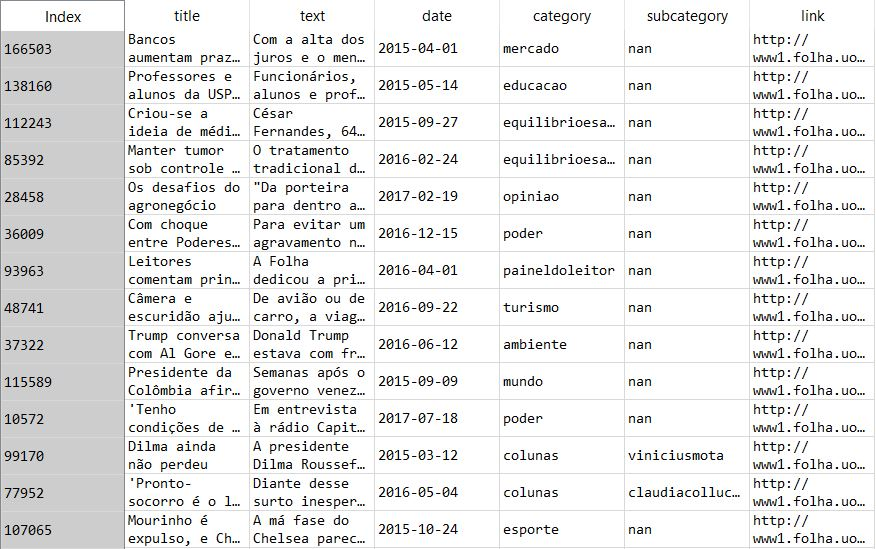
\includegraphics[width=15cm]{folha-dataset}
	  		\caption{Alguns exemplos de notícias encontrados no conjunto de dados do jornal Folha de S. Paulo. A figura mostra todas as colunas disponíveis no conjunto: ``\textit{title}'', ``\textit{text}'', ``\textit{date}'', ``\textit{category}'' e ``\textit{subcategory}''.}
	  		\label{fig:folha-dataset-fig}
	  	\end{figure}
  		\subsection{Pré-processamento de Texto}
  			\paragraph{}Como o conjunto de dados oferecia a informação de categoria da notícia, estes foram filtrados de forma a adquirir apenas as notícias associadas ao mercado, ou seja, onde os valores da coluna ``\textit{category}'' fossem iguais a ``mercado'', o que diminuiu o número total de notícias para 20.970. A coluna ``\textit{subcategory}'' estava vazia em quase todos os registros, tendo apenas o nome do colunista na maioria dos casos diferentes deste. Os artigos não foram removidos, sendo considerados como notícias no conjunto de dados de forma a contribuir para o volume total.
  			\paragraph{}Alguns testes de treino envolvendo apenas o título da notícia foram feitos, estes demonstraram uma baixa taxa de aprendizagem, fazendo com que se preferisse utilizar o processamento do corpo das notícias.
  			\paragraph{}O Núcleo Interinstitucional de Linguística Computacional (NILC) da USP oferece um repositório\cite{nilc-repo} contendo uma série de \textit{embeddings} pré-treinados em português brasileiro. Infelizmente, o repositório encontrava-se em manutenção devido a problemas no servido, o que levou a optar pelo treinamento de \textit{embeddings} nativo do PyText a partir dos dados de treino. Para facilitar e agilizar o treinamentos do \textit{embedding} o corpo das notícias foi pré-processado pelas seguintes etapas:
  			\begin{itemize}
  				\item Normalização para letras minúsculas, para evitar redundâncias.
  				\item Remoção de \textit{stopwords}, palavras como ``a'', ``o'', ``que'' e ``de''.
  				\item \textit{Stemming}, transformação de palavras flexionadas para sua forma radical.
  				\item Remoção e substituição de caracteres especiais.
  			\end{itemize}
  			\paragraph{}Além disso, o formato da coluna de data foi alterada para que esta tivesse a mesma forma da informação de data no conjunto de dados da B3. Por final, as colunas ``\textit{title}'', ``\textit{category}'' e ``\textit{subcategory}'' foram removidas do conjunto.
	  		\begin{figure}[h]
	  			\centering
					{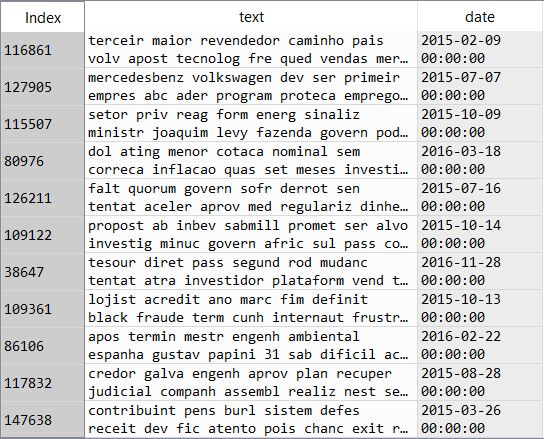
\includegraphics[width=13cm]{folha-pp-dataset}
  				\caption{Exemplos de notícias no conjunto de dados após o pré-processamento.}
  				\label{fig:folha-pp-dataset-fig}}
  			\end{figure}
  			
  	\section{Conjunto de Dados da B3}
  		\paragraph{}Os dados das séries históricas dos ativos pertencentes à B3 pode ser obtido no próprio site da bolsa\cite{b3-serie-historica}. Por conveniência, novamente foi decidido usar um conjunto de dados do Kaggle\cite{b3-dataset}, pois este já agrega os dados oriundos de \cite{b3-serie-historica} entre janeiro de 2000 e maio de 2018, no formato CSV.
			\begin{figure}[h]
				\centering
				{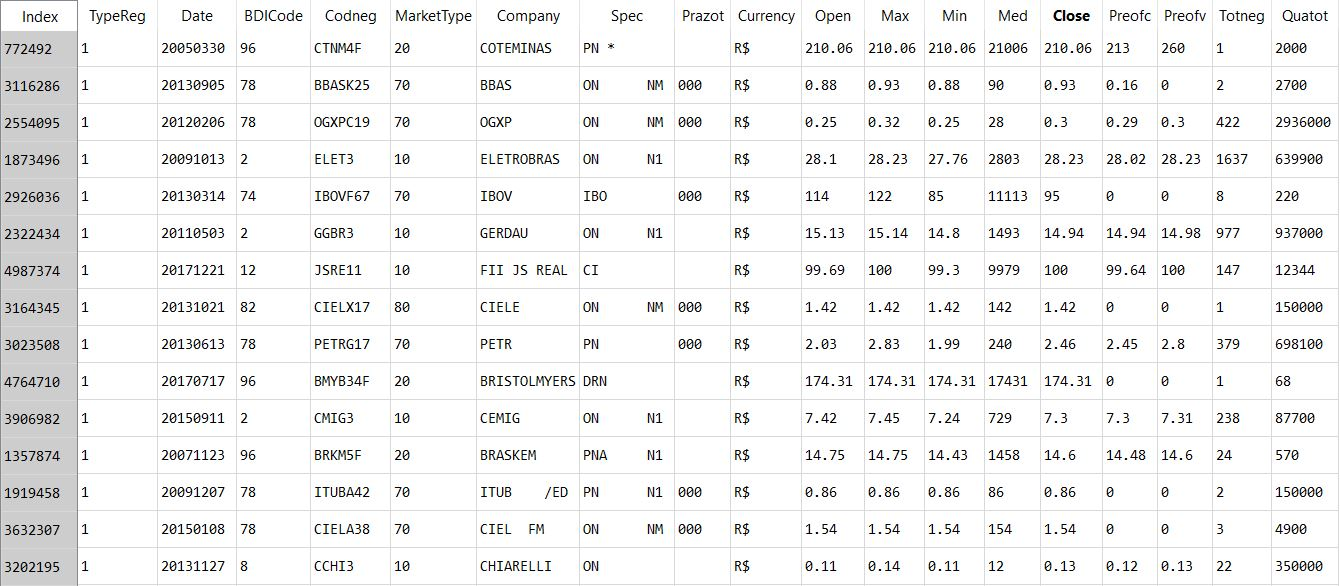
\includegraphics[width=13cm]{b3-dataset}
					\caption{Conjunto de dados da B3 antes do tratamento.}
					\label{fig:b3-dataset-fig}}
			\end{figure}
  		\paragraph{}O primeiro passo dado para tratar os dados foi a remoção de registros que estão fora da mesma janela de tempo que o conjunto de dados das notícias, seguido da seleção dos 5 maiores ativos presentes no iBovespa, como informado na tabela \ref{tab:ibovespa-5bigger}. Além disso, os nomes das colunas foram normalizadas para letras minúsculas e foram preservadas apenas as colunas de código do ativo (\textit{codneg}), preço de fechamento (\textit{close}) e data (\textit{date}).
  		\begin{figure}[h]
  			\centering
  			{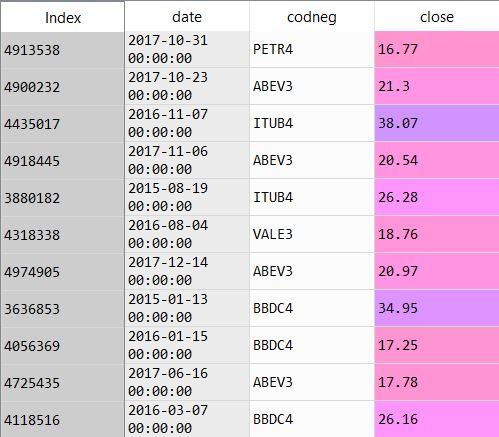
\includegraphics[width=8.5cm]{b3-pp-dataset}
  				\caption{Conjunto de dados da B3 após tratamento.}
  				\label{fig:b3-pp-dataset-fig}}
  		\end{figure}
  	\section{Cruzamento e Conjuntos Finais}
  		\paragraph{}Os conjuntos de dados foram cruzados de forma a obter um conjunto de dados específico para cada combinação de ativo/período de dias. Foi considerado janela de tempo mínima de 1 dia e uma máxima de 5 dias, logo, teríamos $5\times5=25$ conjuntos de dados finais (quantidade de ativos $\times$ número de períodos diferentes).
  		\paragraph{}Sendo assim, um conjunto de dados final relacionaria uma notícia à uma classe que indicaria a valorização de um determinado ativo em uma janela de tempo específica. A classificação foi definida da seguinte forma:
 			\begin{itemize}
  			\item ``1'': Ocorreu valorização, preço de fechamento futuro é maior que o preço de fechamento passado.
	 			\item ``0'': O valor se manteve, preço de fechamento futuro é igual ao preço de fechamento passado.
	 			\item ``-1'': Ocorreu desvalorização, preço de fechamento futuro é menor que o preço de fechamento passado.
  		\end{itemize}
  		\paragraph{}O preço de fechamento passado foi definido como o preço de fechamento do ativo no dia útil anterior ao dia do lançamento da notícia, ao passo que o preço de fechamento futuro foi definido como o preço de fechamento do ativo $X$ dias úteis depois do lançamento da notícia, sendo $X$ um número inteiro de 1 a 5.
  		\begin{figure}[h]
  			\centering
  			{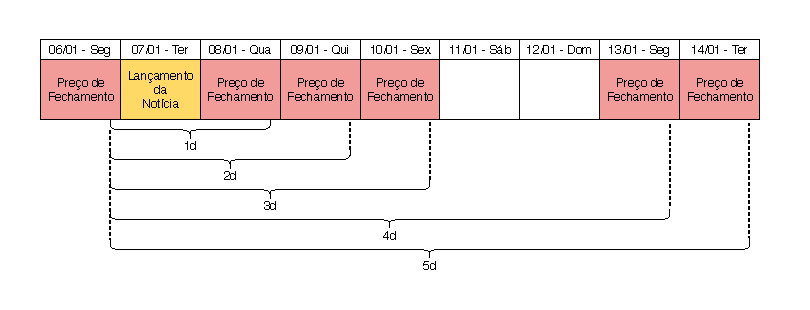
\includegraphics[width=16cm]{calendar-example.pdf}
	 				\caption{Esquema de comparação entre preços de fechamento para a definição da classe de valorização para os intervalos de $1d$(um dia), $2d$(dois dias), $3d$(três dias), $4d$(quatro dias) e $5d$(cinco dias).}
	 				\label{fig:calendar-example-fig}}
  		\end{figure}
  		\begin{figure}[h]
  			\centering
  			{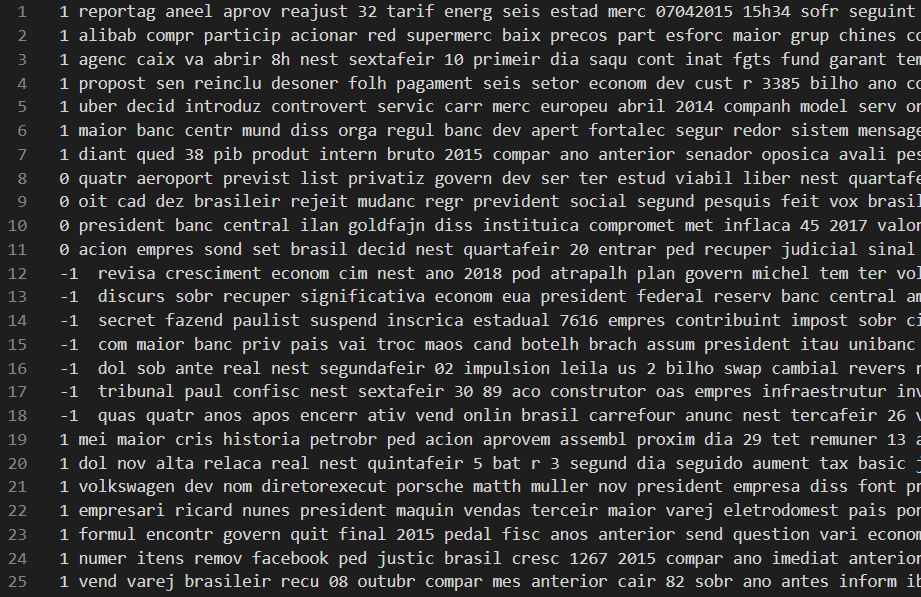
\includegraphics[width=14cm]{abev3_dataset_example}
  				\caption{Exemplo do conjunto de dados criado para o ativo ABEV3 em uma janela de tempo de 1 dia no formato TSV.}
  				\label{fig:abev3_dataset_example-fig}}
  		\end{figure}
  		\paragraph{}Após a criação dos conjuntos de dados para cada dupla de ativo/período, o balanceamento entre classes foi analisado.
  		\begin{table}[h]
  			\caption{Quantidade de registros de cada classe para as combinações de ativo/período.}
  			\label{tab:table-class-balancing}
  			\centering
  			{\footnotesize
  				\begin{tabular}{|c|c|c|c|}
  					\hline
						Conjunto & Classe 1 & Classe 0 & Classe -1 \\
						\hline
						ABEV3/1d & 10912 & 355 & 9679 \\
						ABEV3/2d & 10955 & 235 & 9756 \\
						ABEV3/3d & 10920 & 99 & 9927 \\
						ABEV3/4d & 11081 & 160 & 9705 \\
						ABEV3/5d & 11298 & 343 & 9305 \\
						BBDC4/1d & 10579 & 79 & 10288 \\
						BBDC4/2d & 10282 & 89 & 10575 \\
						BBDC4/3d & 10605 & 24 & 10317 \\
						BBDC4/4d & 11098 & 47 & 9801 \\
						BBDC4/5d & 10954 & 139 & 9853 \\
						ITUB4/1d & 10555 & 49 & 10342 \\
						ITUB4/2d & 10253 & 0 & 10693 \\
						ITUB4/3d & 10474 & 0 & 10472 \\
						ITUB4/4d & 10712 & 54 & 10180 \\
						ITUB4/5d & 10656 & 58 & 10232 \\
						PETR4/1d & 10170 & 222 & 10554 \\
						PETR4/2d & 10581 & 110 & 10255 \\
						PETR4/3d & 10660 & 144 & 10142 \\
						PETR4/4d & 11036 & 89 & 9821 \\
						PETR4/5d & 10910 & 22 & 10014 \\
						VALE3/1d & 10041 & 66 & 10839 \\
						VALE3/2d & 10233 & 81 & 10632 \\
						VALE3/3d & 10473 & 63 & 10410 \\
						VALE3/4d & 10339 & 43 & 10564 \\
						VALE3/5d & 10788 & 111 & 10047 \\
  					\hline
  			\end{tabular}}
  		\end{table}
  		\paragraph{}Como pode ser visto na tabela \ref{tab:table-class-balancing}, os registros da classe 1 e da classe -1 se mostram razoavelmente balanceados, porém, os registros da classe 0 se encontram em mínima quantidade em comparação com as outras duas classes, sendo até inexistente nas combinações ITUB4/2d e ITUB4/3d. Isto pode indicar a alta volatilidade do mercado de ações e a pequena possibilidade do preço de um ativo se manter o mesmo com o passar dos dias.
  		\paragraph{}A possibilidade de utilizar técnicas de \textit{Undersampling} foi descartada devida a mínima quantidade de registros da classe 0. Ao excluir registros da classe 1 e -1, os conjuntos de dados perderiam uma grande parte de informação, o que tornaria a tarefa de classificação textual inviável.
  		\paragraph{}Testes envolvendo \textit{Oversampling} foram feitos, mas os modelos encontrados demonstraram um desempenho pior do que testes feitos sem técnicas de balanceamento. Isto pode ter acontecido pelo fato de que, com o \textit{Oversampling}, a informação de que a classe 0 tem uma menor possibilidade de aparecer nos dados é perdida. Sendo assim, de forma a avaliar o impacto que a classe 0 pode apresentar sobre o treinamento, os conjuntos de dados foram duplicados e os registros da classe 0 foram removidos das cópias. Assim como os conjuntos originais de 3 classes, os conjuntos de 2 classes também foram treinados e analisados. Com isso, o número final de conjunto de dados foi de $25\times2=50$.
  		\paragraph{}Seguindo o princípio de Pareto, todos os conjuntos foram divididos em subconjuntos de treino (80\%) e teste (20\%). Esta proporção foi aplicada separadamente sobre os registros de cada classe para evitar um balanceamento diferente do conjunto de dados original nos subconjuntos de treino e teste.
  		\paragraph{}A rotina de manipulação, pré-processamento e criação dos conjuntos de dados está descrita no apêndice \ref{sec:rotina-de-pre-processamento-e-criacao-de-conjuntos-de-dados}. Foi feita utilizando a linguagem Python com o suporte de bibliotecas como pandas, numpy, csv, nltk e re.
  		
  \chapter{Treinamento e Teste}
	  \paragraph{}Como já dito anteriormente, o treinamento e a geração dos modelos preditivos foram feitos utilizando o framework PyText. Para isso, seria necessário escrever e executar 50 arquivos de configuração. Para evitar este esforço, uma rotina em Python foi desenvolvida para a criação dos arquivos de configuração e da execução destes pelo PyText para todos os conjuntos de dados. A rotina pode ser vista no apêndice \ref{sec:rotina-de-criacao-de-arquivos-de-configuracao-e-execucao-de-treinamentos}.
	  \section{Configuração}
		  \paragraph{}Pela falta do arquivo de \textit{embeddings} pré-treinados e pelas quantias de \textit{epochs} utilizadas, cada treinamento de um conjunto de dados durava uma considerável quantia de tempo (entre 20 e 30 minutos), o que tornou a exploração de todos os parâmetros do PyText muito custosa. No entanto, foi possível realizar testes antes de definir uma configuração mais performática através da escolha do número de \textit{epochs}, tipo de rede neural utilizada e \textit{dropout}.
		  \subsection{Número de \textit{Epochs}}
		  	\paragraph{}O número de \textit{epochs} inicialmente decidido foi de 20, porém, testes mostraram que o modelo apresenta um alto aumento no valor de perda a partir da 12ª \textit{epoch}. Tornando razoável a decisão de usar 10 \textit{epochs}, como o padrão definido pelo PyText.
		  	\paragraph{}Além disso, é notável a perda de acurácia obtida sobre o conjunto de teste após a 10ª \textit{epoch}, provavelmente devido ao sobreajuste em relação ao conjunto de teste com o avanço das \textit{epochs}.
		  	\begin{figure}[H]
		  		\centering
		  		{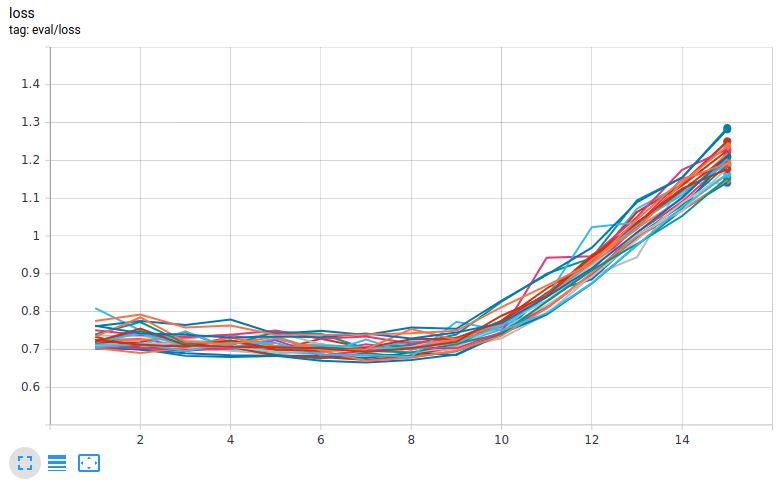
\includegraphics[width=14cm]{loss_graph}
		  			\caption{Gráfico de \textit{loss} gerado pelo TensorBoard, indicando o aumento  da perda a partir da 10ª \textit{epoch}.}
		  			\label{fig:loss_graph-fig}}
		  	\end{figure}
%			 	\begin{figure}[H]
%			 		\centering
%			 		{\includegraphics[width=14cm]{accurancy-graph}
%			 			\caption{Gráfico de \textit{accurancy} gerado pelo TensorBoard, indicando a perda de acurácia a partir da 10ª \textit{epoch}.}
%			 			\label{fig:accurancy-graph-fig}}
%			 	\end{figure}
		  	\paragraph{}Em alguns poucos casos, pode-se verificar um aumento de acurácia após a 10ª \text{epoch}. Logo, foi decidido um meio-termo entre a decisão inicial e o recomendado pelo PyText, optando assim por 20 \textit{epochs}.
		  \subsection{Tipo de Rede}
			  \paragraph{}Testes foram feitos com os dois tipos de redes neurais oferecidas pelo PyText para classificação de texto e mesmo com algumas alterações, a rede CNN obteve melhor performance em comparação a rede BiLSTM, tanto em acurácia quanto tempo de processamento.
			  \paragraph{}TODO: imagem comparativa
			  \paragraph{}Sendo assim, preferiu-se utilizar a rede CNN, o padrão utilizado pelo PyText.
		  \subsection{\textit{Dropout}}
			  \paragraph{}Alguns valores de \textit{dropout} foram testados entre $0,2$ e $0,8$, mas este não demonstraram tanta diferença de performance entre si, tendo um pouco mais de vantagem utilizando $0,6$, o padrão utilizado pelo PyText.
 		\section{Análise}
 			\paragraph{}Tendo as definições de configuração do PyText prontas no modelo de arquivo de configuração (apêndice \ref{sec:modelo-de-arquivo-de-configuracao}), restou executar a rotina para a execução dos testes. Com isto, pode-se obter todas as métricas mencionadas em \ref{sec:metricas} e os arquivos exportados caffe2 de cada modelo preditivo.
 			\paragraph{}Como utilizamos 5 ativos, 5 períodos de tempo e duas variações (uma abrangendo duas classes e outra três classes) foi possível obter ao final 50 modelos preditivos.
 			\subsection{Caso de 3 classes}
	 			\begin{itemize}
	 				\item Maior acurácia: $60,21$ (BBDC4/4d)
	 				\item Menor acurácia: $57,25$ (BBDC4/3d)
	 				\item Média de acurácia para ABEV3: $57,85$
	 				\item Média de acurácia para BBDC4: $58,60$
	 				\item Média de acurácia para ITUB4: $58,13$
	 				\item Média de acurácia para PETR4: $58,00$
	 				\item Média de acurácia para VALE3: $58,10$
	 				\item Média de acurácia para 1 dia: $57,79$
	 				\item Média de acurácia para 2 dias: $56,89$
	 				\item Média de acurácia para 3 dias: $57,86$
	 				\item Média de acurácia para 4 dias: $58,94$
	 				\item Média de acurácia para 5 dias: $58,91$
	 				\item Média de acurácia geral: $58,14$
	 			\end{itemize}
	 			\begin{table}[h]
	 				\caption{Acurácia para o caso de 3 classes.}
	 				\label{tab:3c_ac_analysis}
	 				\centering
	 				{\footnotesize
	 					\begin{tabular}{|c|c|c|c|c|c|}
	 						\hline
	 						\diagbox[linewidth=0.2pt, width=\dimexpr \textwidth/10+2\tabcolsep\relax, height=0.8cm]{Dias}{Ativo}
	 						& ABEV3 & BBDC4 & ITUB4 & PETR4 & VALE3\\
	 						\hline
	 						1 & 57,34 & 57,78 & 58,15 & 57,32 & 58,34 \\
	 						2 & 57,63 & 57,82 & X     & 56,67 & 55,43 \\
	 						3 & 57,96 & 57,25 & X     & 58,27 & 57,97 \\
	 						4 & 58,77 & 60,21 & 57,84 & 58,32 & 59,55 \\
	 						5 & 57,57 & 59,93 & 58,41 & 59,42 & 59,20 \\
	 						\hline
	 				\end{tabular}}
	 			\end{table}
	 			\begin{itemize}
	 				\item Maior precisão média: $72,04$ (PETR4/4d)
	 				\item Menor precisão média: $38,28$ (BBDC4/3d)
	 				\item Média de precisão média para ABEV3: $50,43$
	 				\item Média de precisão média para BBDC4: $39,07$
	 				\item Média de precisão média para ITUB4: $38,82$
	 				\item Média de precisão média para PETR4: $53,10$
	 				\item Média de precisão média para VALE3: $42,10$
	 				\item Média de precisão média para 1 dia: $41,91$
	 				\item Média de precisão média para 2 dias: $51,88$
	 				\item Média de precisão média para 3 dias: $41,37$
	 				\item Média de precisão média para 4 dias: $49,19$
	 				\item Média de precisão média para 5 dias: $42,30$
	 				\item Média de precisão média geral: $45,22$
	 			\end{itemize}
	 			\begin{table}[h]
	 				\caption{Precisão média para o caso de 3 classes.}
	 				\label{tab:3c_pr_analysis}
	 				\centering
	 				{\footnotesize
	 					\begin{tabular}{|c|c|c|c|c|c|}
	 						\hline
	 						\diagbox[linewidth=0.2pt, width=\dimexpr \textwidth/10+2\tabcolsep\relax, height=0.8cm]{Dias}{Ativo}
	 						& ABEV3 & BBDC4 & ITUB4 & PETR4 & VALE3\\
	 						\hline
	 						1 & 38,39 & 38,54 & 38,85 & 54,86 & 38,91 \\
	 						2 & 55,02 & 38,61 & X     & 60,12 & 53,78 \\
	 						3 & 49,65 & 38,28 & X     & 38,82 & 38,72 \\
	 						4 & 55,64 & 40,01 & 38,56 & 72,04 & 39,70 \\
	 						5 & 53,45 & 39,92 & 39,04 & 39,66 & 39,41 \\
	 						\hline
	 				\end{tabular}}
	 			\end{table}
				\begin{itemize}
	 				\item Maior cobertura média: $0$ (BBDC4/4d)
	 				\item Menor cobertura média: $0$ (BBDC4/4d)
	 				\item Média de cobertura média para ABEV3: $0$
	 				\item Média de cobertura média para BBDC4: $0$
	 				\item Média de cobertura média para ITUB4: $0$
	 				\item Média de cobertura média para PETR4: $0$
	 				\item Média de cobertura média para VALE3: $0$
	 				\item Média de cobertura média para 1 dia: $0$
	 				\item Média de cobertura média para 2 dias: $0$
	 				\item Média de cobertura média para 3 dias: $0$
	 				\item Média de cobertura média para 4 dias: $0$
	 				\item Média de cobertura média para 5 dias: $0$
	 				\item Média de cobertura média geral: $0$
	 			\end{itemize}
	 			\begin{table}[h]
	 				\caption{Cobertura média para o caso de 3 classes.}
	 				\label{tab:3c_co_analysis}
	 				\centering
	 				{\footnotesize
	 					\begin{tabular}{|c|c|c|c|c|c|}
	 						\hline
	 						\diagbox[linewidth=0.2pt, width=\dimexpr \textwidth/10+2\tabcolsep\relax, height=0.8cm]{Dias}{Ativo}
	 						& ABEV3 & BBDC4 & ITUB4 & PETR4 & VALE3\\
	 						\hline
	 						1 & 39,04 & 38,69 & 38,81 & 40,04 & 38,72 \\
	 						2 & 39,66 & 38,73 & X     & 40,86 & 39,25 \\
	 						3 & 40,27 & 38,26 & X     & 39,08 & 38,78 \\
	 						4 & 41,15 & 39,80 & 38,66 & 40,62 & 39,78 \\
	 						5 & 41,29 & 39,82 & 39,11 & 39,70 & 39,60 \\
	 						\hline
	 				\end{tabular}}
	 			\end{table}
				\begin{itemize}
	 				\item Maior medida F1: $0$ (BBDC4/4d)
	 				\item Menor medida F1: $0$ (BBDC4/4d)
	 				\item Média de medida F1 para ABEV3: $0$
	 				\item Média de medida F1 para BBDC4: $0$
	 				\item Média de medida F1 para ITUB4: $0$
	 				\item Média de medida F1 para PETR4: $0$
	 				\item Média de medida F1 para VALE3: $0$
	 				\item Média de medida F1 para 1 dia: $0$
	 				\item Média de medida F1 para 2 dias: $0$
	 				\item Média de medida F1 para 3 dias: $0$
	 				\item Média de medida F1 para 4 dias: $0$
	 				\item Média de medida F1 para 5 dias: $0$
	 				\item Média de medida F1 geral: $0$
	 			\end{itemize}
	 			\begin{table}[h]
	 				\caption{Medida F1 média para o caso de 3 classes.}
	 				\label{tab:3c_f1_analysis}
	 				\centering
	 				{\footnotesize
	 					\begin{tabular}{|c|c|c|c|c|c|}
	 						\hline
	 						\diagbox[linewidth=0.2pt, width=\dimexpr \textwidth/10+2\tabcolsep\relax, height=0.8cm]{Dias}{Ativo}
	 						& ABEV3 & BBDC4 & ITUB4 & PETR4 & VALE3\\
	 						\hline
	 						1 & 38,55 & 38,59 & 38,63 & 41,07 & 38,43 \\
	 						2 & 40,28 & 38,64 & X     & 42,73 & 40,62 \\
	 						3 & 41,39 & 38,13 & X     & 38,94 & 38,64 \\
	 						4 & 42,58 & 39,67 & 38,61 & 42,18 & 39,74 \\
	 						5 & 42,71 & 39,53 & 38,97 & 39,63 & 39,50 \\
	 						\hline
	 				\end{tabular}}
	 			\end{table}
			\subsection{Caso de 2 classes}
				\begin{itemize}
	 				\item Maior acurácia: $0$ (BBDC4/4d)
	 				\item Menor acurácia: $0$ (BBDC4/4d)
	 				\item Média de acurácia para ABEV3: $0$
	 				\item Média de acurácia para BBDC4: $0$
	 				\item Média de acurácia para ITUB4: $0$
	 				\item Média de acurácia para PETR4: $0$
	 				\item Média de acurácia para VALE3: $0$
	 				\item Média de acurácia para 1 dia: $0$
	 				\item Média de acurácia para 2 dias: $0$
	 				\item Média de acurácia para 3 dias: $0$
	 				\item Média de acurácia para 4 dias: $0$
	 				\item Média de acurácia para 5 dias: $0$
	 				\item Média de acurácia geral: $0$
	 			\end{itemize}
	 			\begin{table}[h]
	 				\caption{Acurácia para o caso de 2 classes.}
	 				\label{tab:2c_ac_analysis}
	 				\centering
	 				{\footnotesize
	 					\begin{tabular}{|c|c|c|c|c|c|}
	 						\hline
	 						\diagbox[linewidth=0.2pt, width=\dimexpr \textwidth/10+2\tabcolsep\relax, height=0.8cm]{Dias}{Ativo}
	 						& ABEV3 & BBDC4 & ITUB4 & PETR4 & VALE3\\
	 						\hline
	 						1 & 58,74 & 56,71 & 57,72 & 56,12 & 57,16 \\
	 						2 & 56,16 & 57,61 & 57,83 & 56,71 & 57,54 \\
	 						3 & 59,46 & 59,25 & 58,25 & 57,48 & 57,07 \\
	 						4 & 57,71 & 58,32 & 60,08 & 58,26 & 58,17 \\
	 						5 & 58,97 & 60,52 & 59,61 & 59,33 & 59,37 \\
	 						\hline
	 				\end{tabular}}
	 			\end{table}
				\begin{itemize}
	 				\item Maior precisão média: $0$ (BBDC4/4d)
	 				\item Menor precisão média: $0$ (BBDC4/4d)
	 				\item Média de precisão média para ABEV3: $0$
	 				\item Média de precisão média para BBDC4: $0$
	 				\item Média de precisão média para ITUB4: $0$
	 				\item Média de precisão média para PETR4: $0$
	 				\item Média de precisão média para VALE3: $0$
	 				\item Média de precisão média para 1 dia: $0$
	 				\item Média de precisão média para 2 dias: $0$
	 				\item Média de precisão média para 3 dias: $0$
	 				\item Média de precisão média para 4 dias: $0$
	 				\item Média de precisão média para 5 dias: $0$
	 				\item Média de precisão média geral: $0$
	 			\end{itemize}
	 			\begin{table}[h]
	 				\caption{Precisão média para o caso de 2 classes.}
	 				\label{tab:2c_pr_analysis}
	 				\centering
	 				{\footnotesize
	 					\begin{tabular}{|c|c|c|c|c|c|}
	 						\hline
	 						\diagbox[linewidth=0.2pt, width=\dimexpr \textwidth/10+2\tabcolsep\relax, height=0.8cm]{Dias}{Ativo}
	 						& ABEV3 & BBDC4 & ITUB4 & PETR4 & VALE3\\
	 						\hline
	 						1 & 58,97 & 56,93 & 57,73 & 56,10 & 57,04 \\
	 						2 & 56,16 & 57,62 & 57,91 & 56,79 & 57,58 \\
	 						3 & 59,38 & 59,24 & 58,30 & 57,49 & 57,08 \\
	 						4 & 57,73 & 58,04 & 60,35 & 58,28 & 58,16 \\
	 						5 & 58,43 & 60,62 & 59,61 & 59,25 & 59,31 \\
	 						\hline
	 				\end{tabular}}
	 			\end{table}
				\begin{itemize}
	 				\item Maior cobertura média: $0$ (BBDC4/4d)
	 				\item Menor cobertura média: $0$ (BBDC4/4d)
	 				\item Média de cobertura média para ABEV3: $0$
	 				\item Média de cobertura média para BBDC4: $0$
	 				\item Média de cobertura média para ITUB4: $0$
	 				\item Média de cobertura média para PETR4: $0$
	 				\item Média de cobertura média para VALE3: $0$
	 				\item Média de cobertura média para 1 dia: $0$
	 				\item Média de cobertura média para 2 dias: $0$
	 				\item Média de cobertura média para 3 dias: $0$
	 				\item Média de cobertura média para 4 dias: $0$
	 				\item Média de cobertura média para 5 dias: $0$
	 				\item Média de cobertura média geral: $0$
	 			\end{itemize}
	 			\begin{table}[h]
		 				\caption{Cobertura média para o caso de 2 classes.}
		 				\label{tab:2c_co_analysis}
		 				\centering
		 				{\footnotesize
		 					\begin{tabular}{|c|c|c|c|c|c|}
		 						\hline
		 						\diagbox[linewidth=0.2pt, width=\dimexpr \textwidth/10+2\tabcolsep\relax, height=0.8cm]{Dias}{Ativo}
		 						& ABEV3 & BBDC4 & ITUB4 & PETR4 & VALE3\\
		 						\hline
		 						1 & 58,97 & 56,80 & 57,67 & 55,99 & 56,82 \\
		 						2 & 56,18 & 57,62 & 57,89 & 56,76 & 57,57 \\
		 						3 & 58,97 & 59,21 & 58,25 & 57,50 & 57,07 \\
		 						4 & 57,76 & 59,28 & 59,78 & 58,30 & 58,16 \\
		 						5 & 58,32 & 60,64 & 59,51 & 59,24 & 59,12 \\
		 						\hline
		 				\end{tabular}}
		 			\end{table}
					\begin{itemize}
						\item Maior medida F1: $0$ (BBDC4/4d)
						\item Menor medida F1: $0$ (BBDC4/4d)
						\item Média de medida F1 para ABEV3: $0$
						\item Média de medida F1 para BBDC4: $0$
						\item Média de medida F1 para ITUB4: $0$
						\item Média de medida F1 para PETR4: $0$
						\item Média de medida F1 para VALE3: $0$
						\item Média de medida F1 para 1 dia: $0$
						\item Média de medida F1 para 2 dias: $0$
						\item Média de medida F1 para 3 dias: $0$
						\item Média de medida F1 para 4 dias: $0$
						\item Média de medida F1 para 5 dias: $0$
						\item Média de medida F1 geral: $0$
					\end{itemize}
		 			\begin{table}[h]
		 				\caption{Medida F1 média para o caso de 2 classes.}
		 				\label{tab:2c_f1_analysis}
		 				\centering
		 				{\footnotesize
		 					\begin{tabular}{|c|c|c|c|c|c|}
		 						\hline
		 						\diagbox[linewidth=0.2pt, width=\dimexpr \textwidth/10+2\tabcolsep\relax, height=0.8cm]{Dias}{Ativo}
		 						& ABEV3 & BBDC4 & ITUB4 & PETR4 & VALE3\\
		 						\hline
		 						1 & 58,74 & 56,54 & 57,61 & 55,84 & 56,63 \\
		 						2 & 56,12 & 57,61 & 57,82 & 56,68 & 57,53 \\
		 						3 & 58,76 & 59,19 & 58,18 & 57,47 & 57,05 \\
		 						4 & 57,67 & 57,83 & 59,39 & 58,23 & 58,15 \\
		 						5 & 58,33 & 60,52 & 59,45 & 59,25 & 59,03 \\
		 						\hline
		 				\end{tabular}}
		 			\end{table}
  
  \chapter{Considerações Finais}
  	\paragraph{}TODO
  	\section{Conclusão}
  		\paragraph{}TODO
 		\section{Trabalhos Futuros}
 			\paragraph{}TODO

  \backmatter
  \bibliographystyle{coppe-unsrt}
  \bibliography{bibliography}

  \appendix	

	\chapter{Rotinas e Arquivos de Configuração}
		\section{Rotina de Pré-processamento e Criação de Conjuntos de Dados}\label{sec:rotina-de-pre-processamento-e-criacao-de-conjuntos-de-dados}
			\begin{minted}[frame=leftline,
			linenos=true,
			fontsize=\small,
			breaklines]{python}
import re
import numpy as np
import pandas as pd
import csv
import os
from datetime import timedelta
from unicodedata import normalize
import nltk
nltk.download('stopwords')
from nltk.corpus import stopwords
from nltk.stem.snowball import SnowballStemmer

OUT_DIR = './dataset_out'
MAX_DAYS = 5
TRAIN_PERCENTAGE_SIZE = 80/100
TEST_PERCENTAGE_SIZE = 20/100
REGEXP_REMOVE_SPECIAL = re.compile('[^a-zA-Z0-9 ]+')
ONLY_ONE_CODE = False
ONLY_ONE_CODE_NAME = 'VALE3'
STOPWORDS = stopwords.words('portuguese')
STEMMER = SnowballStemmer('portuguese')
ARTIGOS_TEXT_COLUMN = 'text'
ARTIGOS_UNUSED_COLUMNS = ['title', 'category', 'subcategory', 'link']
BOVESPA_UNUSED_COLUMNS = ['open', 'company', 'typereg', 'bdicode', 'markettype', 'spec', 'prazot', 'currency', 'max', 'min', 'med', 'preofc', 'preofv', 'totneg', 'quatot']

df_companies = pd.read_csv('../datasets/company-codes.csv')
df_bovespa = pd.read_csv('../datasets/kaggle/bovespa.csv')
df_articles = pd.read_csv('../datasets/kaggle/articles.csv')

def getAppreciation(before, after):
  if after > before:
    return 1
  if before > after:
    return -1
  else:
    return 0

def getEffectDate(date):
  effectDate = date
  while (df_bovespa[df_bovespa.date == effectDate].size < 1):
    effectDate = effectDate + timedelta(days=1)
  return effectDate

def exportToTSV(dataframe, filename):
  if not os.path.exists(OUT_DIR):
    os.mkdir(OUT_DIR)
  fullpath = '%s/%s' % (OUT_DIR, filename)
  dataframe.to_csv(fullpath, sep='\t', quoting=csv.QUOTE_NONE, index=False, header=False)

def getCleanText(text):
  finalTextArray = []
  lowerText = text.lower()
  for word in lowerText.split():
    if word not in STOPWORDS:
      finalTextArray.append(STEMMER.stem(word))
  finalText = ' '.join(finalTextArray)
  finalText = normalize('NFKD', finalText).encode('ASCII', 'ignore').decode('ASCII')
  finalText = REGEXP_REMOVE_SPECIAL.sub('', finalText)
  finalText = re.sub(' +', ' ', finalText)
  return finalText

df_articles = df_articles[df_articles.category == 'mercado']
df_articles.drop(ARTIGOS_UNUSED_COLUMNS, inplace=True, axis=1)
df_articles['date'] = df_articles.apply(lambda row: np.int64(row['date'].replace('-', '')), axis=1)
df_articles['date'] = pd.to_datetime(df_articles['date'].astype(str), format='%Y%m%d')

df_bovespa.columns = map(str.lower, df_bovespa.columns)
df_bovespa = df_bovespa[df_bovespa.codneg.str.strip().isin(df_companies.code)]
df_bovespa['date'] = pd.to_datetime(df_bovespa['date'].astype(str), format='%Y%m%d')
df_bovespa = df_bovespa[df_bovespa.date >= df_articles.date.min()]
df_bovespa.drop(BOVESPA_UNUSED_COLUMNS, inplace=True, axis=1)
df_bovespa = df_bovespa.sort_values('date')

df_articles['date'] = df_articles.apply(lambda row: getEffectDate(row.date), axis=1)
df_articles[ARTIGOS_TEXT_COLUMN] = df_articles.apply(lambda row: getCleanText(row[ARTIGOS_TEXT_COLUMN]), axis=1)
df_articles = df_articles.sort_values('date')

df_analysis = pd.DataFrame(columns=['dataset','1s','0s', '-1s'])

for index, row in df_companies.iterrows():
  if not ONLY_ONE_CODE or (ONLY_ONE_CODE and row['code'] == ONLY_ONE_CODE_NAME):
    print('Generating for ' + row['code'])
    df_full = df_bovespa[df_bovespa.codneg.str.strip() == row['code']]
    df_full = df_full.assign(close_before=df_full['close'].transform(lambda group: group.shift(1)))
    df_full = df_full[~np.isnan(df_full.close_before)]
    for d in range(MAX_DAYS):
      interval = d + 1
      df_interval = df_full.assign(close_after=df_full['close'].transform(lambda group: group.shift(-interval)))
      df_interval = df_interval[~np.isnan(df_interval.close_after)]
      df_interval.drop('close', inplace=True, axis=1)
      df_company = pd.merge(df_articles, df_interval, on='date', how='inner')
      if df_company.size > 0:
        df_company.drop(['date', 'codneg'], inplace=True, axis=1)
        df_company['label'] = df_company.apply(lambda row: getAppreciation(row['close_before'], row['close_after']), axis=1)
        df_company.drop(['close_before', 'close_after'], inplace=True, axis=1)
        df_company = df_company[['label', ARTIGOS_TEXT_COLUMN]]
        
        df_company_positive = df_company[df_company.label == 1].sample(frac=1)
        df_company_neutral = df_company[df_company.label == 0].sample(frac=1)
        df_company_negative = df_company[df_company.label == -1].sample(frac=1)

        analysis = pd.Series({"dataset": row['code'] + '_' + str(interval) + 'd.tsv', "1s": len(df_company_positive), "0s": len(df_company_neutral), "-1s": len(df_company_negative)})
        df_analysis = df_analysis.append(analysis, ignore_index=True)
        
        trainPositiveSize = round(len(df_company_positive)*(TRAIN_PERCENTAGE_SIZE))
        testPositiveSize = round(len(df_company_positive)*(TEST_PERCENTAGE_SIZE))

        trainNeutralSize = round(len(df_company_neutral)*(TRAIN_PERCENTAGE_SIZE))
        testNeutralSize = round(len(df_company_neutral)*(TEST_PERCENTAGE_SIZE))

        trainNegativeSize = round(len(df_company_negative)*(TRAIN_PERCENTAGE_SIZE))
        testNegativeSize = round(len(df_company_negative)*(TEST_PERCENTAGE_SIZE))
        
        df_company_train = df_company_positive.head(trainPositiveSize)
        df_company_positive = df_company_positive.iloc[trainPositiveSize:]
        df_company_train = df_company_train.append(df_company_negative.head(trainNegativeSize))
        df_company_negative = df_company_negative.iloc[trainNegativeSize:]

        df_company_test = df_company_positive.head(testPositiveSize)
        df_company_positive = df_company_positive.iloc[testPositiveSize:]
        df_company_test = df_company_test.append(df_company_negative.head(testNegativeSize))
        df_company_negative = df_company_negative.iloc[testNegativeSize:]

        exportToTSV(df_company_train, row['code'] + '_2c_' + str(interval) + 'd_train.tsv')
        exportToTSV(df_company_test, row['code'] + '_2c_' + str(interval) + 'd_test.tsv')

        df_company_train = df_company_train.append(df_company_neutral.head(trainNeutralSize))
        df_company_neutral = df_company_neutral.iloc[trainNeutralSize:]
        df_company_test = df_company_test.append(df_company_neutral.head(testNeutralSize))
        df_company_neutral = df_company_neutral.iloc[testNeutralSize:]
        
        exportToTSV(df_company_train, row['code'] + '_3c_' + str(interval) + 'd_train.tsv')
        exportToTSV(df_company_test, row['code'] + '_3c_' + str(interval) + 'd_test.tsv')
			\end{minted}
		\section{Rotina de Criação de Arquivos de Configuração e Execução de Treinamentos}\label{sec:rotina-de-criacao-de-arquivos-de-configuracao-e-execucao-de-treinamentos}
			\begin{minted}[frame=leftline,
			linenos=true,
			fontsize=\small,
			breaklines]{python}
import os
import pandas as pd
import subprocess
import glob

MAX_DAYS = 5
df_companies = pd.read_csv("../datasets/company-codes.csv")

for index, row in df_companies.iterrows():
  asset = row['code']
  for d in range(MAX_DAYS):
    interval = d + 1
    # configName = asset + "_2c_" + str(interval) + "d"
    configName = asset + "_3c_" + str(interval) + "d"
    fileName = "configs/" + configName + ".json"
    with open("templateconfig_XXXXX_Yc_Zd.json") as inputFile, open(fileName, "w") as outputFile:
      for line in inputFile:
        outputFile.write(line.replace("XXXXX_Yc_Zd", configName))

    print("Executing for " + configName)

    bashCommand = "pytext train < " + fileName
    result = subprocess.run(bashCommand, shell=True, stdout=subprocess.PIPE)
    result.stdout.decode('utf-8')

    print("Renaming run folder")

    runFoldersList = glob.glob("runs/*")
    latestRunFolder = max(runFoldersList, key=os.path.getctime)
    os.rename(latestRunFolder, "runs/" + configName)

    print("Execution done for " + configName)
			\end{minted}
		\section{Modelo de Arquivo de Configuração}\label{sec:modelo-de-arquivo-de-configuracao}
			\begin{minted}[frame=leftline,
			linenos=true,
			fontsize=\small,
			breaklines]{json}
{
  "version": 18,
  "task": {
    "DocumentClassificationTask": {
      "data": {
        "source": {
          "TSVDataSource": {
            "field_names": ["label", "text"],
            "train_filename": "../preprocessor/dataset_out/XXXXX_Yc_Zd_train.tsv",
            "test_filename": "../preprocessor/dataset_out/XXXXX_Yc_Zd_test.tsv",
            "eval_filename": "../preprocessor/dataset_out/XXXXX_Yc_Zd_test.tsv"
          }
        }
      },
      "model": {
        "DocModel": {
          "representation": {
            "DocNNRepresentation": {}
          }
        }
      },
      "trainer": {
        "epochs": 15
      },
      "metric_reporter": {
        "output_path": "metric_reports/XXXXX_Yc_Zd.txt",
        "model_select_metric": "accuracy",
        "target_label": null,
        "text_column_names": [
          "text"
        ]
      }
    }
  },
  "export_torchscript_path": "torchscripts/XXXXX_Yc_Zd.pt1",
  "export_caffe2_path": "caffe2_exports/XXXXX_Yc_Zd.caffe2.predictor"
}
			\end{minted}
		\section{Arquivo com Lista de Ativos a Serem Processados}
					\begin{minted}[frame=leftline,
					linenos=true,
					fontsize=\small,
					breaklines]{text}
code,names
ABEV3,AMBEV
BBDC4,BRADESCO
ITUB4,ITAU
PETR4,PETROBRAS
VALE3,Vale
					\end{minted}

\end{document}
%% 
%%
%% End of file `example.tex'.
